\documentclass[10pt,letterpaper]{article}

\usepackage[T1]{fontenc}
\usepackage[utf8]{inputenc}
\usepackage{newtxtext}
\usepackage{newtxmath}
\usepackage[margin=0.76in,top=0.78in,bottom=0.78in]{geometry}
\usepackage{amsmath,mathtools}
\usepackage{microtype}
\usepackage{graphicx}
\usepackage{booktabs}
\usepackage{array}
\usepackage{tabularx}
\usepackage{multirow}
\usepackage[table]{xcolor}
\usepackage{enumitem}
\usepackage{fancyhdr}
\usepackage{titlesec}
\usepackage{placeins}
\usepackage[numbers,sort&compress]{natbib}
\usepackage[colorlinks=true,linkcolor=navy,citecolor=navy,urlcolor=navy]{hyperref}

\definecolor{navy}{HTML}{1B4F72}
\definecolor{tealdark}{HTML}{145A32}
\definecolor{greenbg}{HTML}{EAFAF1}
\definecolor{reddark}{HTML}{922B21}
\definecolor{redbg}{HTML}{FDEDEC}
\definecolor{amberdark}{HTML}{7D6608}
\definecolor{amberbg}{HTML}{FEF9E7}
\definecolor{slate}{HTML}{34495E}
\definecolor{lightgray}{HTML}{F4F6F7}
\definecolor{bordergray}{HTML}{BDC3C7}

\titleformat{\section}{\large\bfseries\color{navy}}{\thesection.}{0.55em}{}[\vspace{-0.4em}\color{bordergray}\rule{\linewidth}{0.6pt}]
\titleformat{\subsection}{\normalsize\bfseries\color{slate}}{\thesubsection}{0.5em}{}
\titlespacing*{\section}{0pt}{13pt}{5.5pt}
\titlespacing*{\subsection}{0pt}{8.5pt}{3pt}

\pagestyle{fancy}
\fancyhf{}
\fancyhead[L]{\footnotesize\color{slate}\textsc{V15 Paper 2 Feasibility Analysis --- PVB Classical \& Quantum Photonics}}
\fancyhead[R]{\footnotesize\color{slate}November 2026}
\fancyfoot[C]{\footnotesize\thepage}
\renewcommand{\headrulewidth}{0.4pt}

\newcommand{\abs}[1]{\lvert #1 \rvert}
\newcommand{\norm}[1]{\lVert #1 \rVert}
\newcommand{\ket}[1]{\lvert #1 \rangle}
\newcommand{\bra}[1]{\langle #1 \rvert}
\newcommand{\braket}[2]{\langle #1 | #2 \rangle}

\begin{document}

\begin{center}
  {\LARGE\bfseries\color{navy} Feasibility Analysis of V15 Paper 2:}\\[4pt]
  {\Large\bfseries\color{slate} Classical and Quantum Photonic Protocols Based on Physical Perfect Vortex Beam Frames}\\[8pt]
  {\small\color{slate}
    \textbf{Author:} Sebasti\'an Ayala (ORCID: \texttt{0009-0003-7348-3883}) \quad$|$\quad
    \textbf{Baseline:} Post-APS Triage Audit of V14 (\texttt{AY13053}) \\[2pt]
    \textbf{Open-Access Library:} 17 verified arXiv PDFs downloaded; 37 clean photonics BibTeX entries \quad$|$\quad
    \textbf{Date:} November 24, 2026
  }
\end{center}
\vspace{4pt}

\noindent\fcolorbox{tealdark}{greenbg}{%
\begin{minipage}{\dimexpr\linewidth-2\fboxsep-2\fboxrule\relax}
\vspace{3pt}
\textbf{\color{tealdark}\large EXECUTIVE VERDICT: HIGHLY FEASIBLE (\textsc{STRONG GO} AS A SEQUENTIAL STANDALONE PAPER FOR \emph{JOURNAL OF OPTICS} OR \emph{JOSA B})}\\[4pt]
\small
V14 Part~II (\texttt{AY13053}) was desk-rejected 1~minute after Part~I because it shared the same AI/HITL triage flags, depended on an unpublished companion paper, and spread itself thin across five short numerical exercises. Moving the noisy $\mathrm{LG}_{2,1}$ Tikhonov benchmark into V15 Paper~1 allows V15 Paper~2 to focus cleanly on \textbf{four deeply engineered, referee-proof photonic protocols}, submitted \emph{after} Paper~1 is live on arXiv:
\begin{itemize}[leftmargin=1.4em,itemsep=2pt,topsep=3pt]
  \item \textbf{Protocol 1 (Step-Index \& Parabolic GRIN RCFs + Tolerances + SDM):} Adding an exact parabolic graded-index (GRIN) RCF solver matches Villalba \emph{et al.}~\cite{Villalba2023}'s guided $l = 0\text{--}6$ window directly from first principles ($n_{\mathrm{eff}}(6)=1.4476 > n_{\mathrm{clad}}$, $99.11\%$ mean PVB coupling, $+6.97\,\mathrm{dB}$ gain over fixed-collimator LG at $l=4$ vs.\ $+6.83\,\mathrm{dB}$ experiment), while quantifying realistic $\delta R, \delta w, \delta x$ launch tolerances.
  \item \textbf{Protocol 2 (Turbulence Filtering vs.\ Matched-Dimension $N=5$ LG \& Multi-Screen Propagation):} Even against an \emph{optimally waist-tuned} ($w_0 = 0.405\,\mathrm{mm}$, $99.74\%$ clean signal capture) $N=5$ single-OAM $\mathrm{LG}_{p,1}$ projector, our $N=5$ discrete PVB dual-frame projector achieves lower field MSE at every turbulence strength ($5.77\times$ over raw and $1.08\text{--}2.97\times$ over $\mathrm{LG}_5$ on single screens; $3.82\text{--}7.70\times$ over raw on 5-screen split-step volume turbulence).
  \item \textbf{Protocol 3 (Gouy IC-POVM Extended Beyond $\mathbb{I}_4/4$):} Correcting V14's $\sigma_m^{+1}$ analyzer scaling and benchmarking $R\hat{\rho}R$ MLE on coherent radial superpositions ($F = 0.9823$ at $N_{\mathrm{phot}} = 10^4$), 20 Haar-random pure radial qudits (mean $F = 0.9922$, min $0.9833$), and uncalibrated axial positioning errors ($\delta z/z_R \le 5\%$ preserves $F \ge 0.972$) transforms Protocol~3 into a realistic experimental proposal.
  \item \textbf{Protocol 4 (Detection-Loophole Iris Threshold \& Fair LG Comparison):} Sweeping $R_{\mathrm{iris}}/R_0$ proves PVBs clear the symmetric CHSH detection-loophole threshold ($\eta_{\mathrm{crit}} = 82.84\%$) at $R_{\mathrm{iris}} = \mathbf{1.048\,R_0}$ (reaching $99.99\%$ two-photon survival at $1.20\,R_0$), compared to $1.324\,R_0$ ($l=4$-matched LG), $1.873\,R_0$ (geometric-mean LG), and $2.649\,R_0$ ($l=1$-matched LG) --- a $1.60\times\text{--}6.39\times$ pupil-area reduction.
\end{itemize}
\vspace{2pt}
\end{minipage}}

\vspace{4pt}

\section{Open-Access Literature Audit and Protocol Grounding}
\label{sec:p2_lit}

All 6 AI-meta citations from V14 Part~II have been removed and replaced by \textbf{17 verified open-access arXiv PDFs} downloaded into \texttt{Paper PVB/V15/Paper 2/References/} alongside a clean 37-entry database (\texttt{references\_v15\_paper2.bib}). Table~\ref{tab:p2_refs} links these open-access anchors directly to the four upgraded photonic protocols.

\begin{table}[t]
\centering
\caption{Curated open-access arXiv literature downloaded into \texttt{V15/Paper 2/References/} (17 verified PDFs) grouped by protocol.}
\label{tab:p2_refs}
\scriptsize
\renewcommand{\arraystretch}{1.15}
\begin{tabularx}{\linewidth}{@{}l>{\raggedright\arraybackslash}p{4.6cm}>{\raggedright\arraybackslash}X@{}}
\toprule
\textbf{Protocol} & \textbf{Open-Access Reference (arXiv / Journal)} & \textbf{Role in Strengthening V15 Paper~2} \\
\midrule
\multirow{3}{*}{\textbf{I. RCF \& SDM}}
  & Villalba, Ayala \emph{et al.} (2023)~\cite{Villalba2023} (\texttt{2308.11354}); Rojas-Rojas \emph{et al.} (2021)~\cite{RojasRojas2021} (\texttt{2101.06280}) & Experimental ($+6.83\,\mathrm{dB}$ at $l=4$, $l=1\text{--}6$) and theoretical ($>99.5\%$) PVB--RCF coupling benchmarks. \\
  & Zhang \emph{et al.} (2018)~\cite{Zhang2018GRIN} (\texttt{1711.04646}); Asgharzadeh \emph{et al.} (2026)~\cite{Asgharzadeh2026} (\texttt{2608.10683}) & Graded-index (GRIN) RCF OAM transmission and 2026 dual-boundary coupling stability analysis motivating our new GRIN solver. \\
  & Fontaine \emph{et al.} (2019)~\cite{Fontaine2019} (\texttt{1803.04126}); Fu \emph{et al.} (2018)~\cite{Fu2018} (\texttt{1809.10319}) & Unitary MPLC and scalable radial mode sorters implementing concentric multi-ring PVB demultiplexing. \\
\midrule
\multirow{2}{*}{\textbf{II. Turbulence}}
  & Roux (2011)~\cite{Roux2011} (\texttt{1009.1956}, \emph{PRA}) & Infinitesimal split-step propagation theory of OAM turbulence decoherence anchoring our new 5-screen volume turbulence test. \\
  & Hamadou Ibrahim \emph{et al.} (2013)~\cite{Ibrahim2013} (\texttt{1306.6495}, \emph{PRA}) & Experimental/numerical Kolmogorov crosstalk statistics for OAM modes ($D/r_0$ scaling). \\
\midrule
\multirow{3}{*}{\textbf{III. Radial IC-POVM}}
  & Gu \emph{et al.} (2018)~\cite{Gu2018} (\texttt{1712.02892}, \emph{PRL}); Zhou \emph{et al.} (2017, 2019)~\cite{Zhou2017,Zhou2019} (\texttt{1711.08120}, \texttt{1809.09986}) & Experimental Gouy-phase and FrFT radial mode sorters demonstrating feasibility of multi-plane radial quantum optics. \\
  & Choudhary \emph{et al.} (2018)~\cite{Choudhary2018} (\texttt{1809.07980}, \emph{Opt.\ Lett.}) & Phase-retrieval radial-mode spectrum measurement providing direct state-of-the-art context for passive Gouy IC-POVM tomography. \\
  & Renes \emph{et al.} (2004)~\cite{Renes2004} (\texttt{quant-ph/0310075}); Lvovsky (2004)~\cite{Lvovsky2004} (\texttt{quant-ph/0311097}) & Foundational IC-POVM frame bounds and $R\hat{\rho}R$ iterative maximum-likelihood tomography algorithm. \\
\midrule
\multirow{2}{*}{\textbf{IV. Iris Bell--CHSH}}
  & Walborn \emph{et al.} (2010)~\cite{Walborn2010} (\texttt{1010.1236}); Ca\~nas \emph{et al.} (2021)~\cite{Canas2021} (\texttt{2109.03064}) & SPDC spatial correlations, aperture truncation, and entangled photon coupling in RCFs. \\
  & V\'ertesi, Pironio \& Brunner (2010)~\cite{Vertesi2010} (\texttt{0909.3171}, \emph{PRL}) & Detection-loophole efficiency thresholds in high-dimensional Bell tests (paired with Eberhard~\cite{Eberhard1993}). \\
\bottomrule
\end{tabularx}
\end{table}

\section{First-Principles Verification of All Four Upgraded Protocols}
\label{sec:p2_verify}

Every new upgrade for V15 Paper~2 has been executed and audited in \texttt{verify\_paper2\_v15.py} (4/4 test suites passed; full JSON archive in \texttt{verify\_paper2\_v15\_results.json}). Table~\ref{tab:p2_results} and Fig.~\ref{fig:p2_feas} document the verified referee-proofing breakthroughs.

\begin{table}[t]
\centering
\caption{Quantitative summary of all four V15 Paper~2 referee-proofing upgrades (\texttt{verify\_paper2\_v15.py}, 4/4 suites passed).}
\label{tab:p2_results}
\scriptsize
\renewcommand{\arraystretch}{1.14}
\begin{tabularx}{\linewidth}{@{}l>{\raggedright\arraybackslash}p{4.5cm}>{\raggedright\arraybackslash}X@{}}
\toprule
\textbf{Protocol} & \textbf{V14 Vulnerability Fixed} & \textbf{Verified V15 Numerical Result} \\
\midrule
\textbf{1. RCF + SDM} & Only step-index fiber modeled vs.\ Villalba's GRIN RCF; no alignment tolerances. & Parabolic GRIN RCF ($r_{\mathrm{mid}}=7.5\,\mu\mathrm{m}, a=1.5\,\mu\mathrm{m}, \Delta n=0.033$) guides $l=0\text{--}6$ ($n_{\mathrm{eff}}(6)=1.4476 > 1.444$, matching Villalba's $l=1\text{--}6$ range!) with \textbf{99.11\% mean PVB coupling} ($w_{\mathrm{opt}}=1.959\,\mu\mathrm{m}$) and \textbf{+6.97\,dB} gain over LG at $l=4$. Coupling stays $>92\%$ for $\abs{\delta x}\le 0.5\,\mu\mathrm{m}$ lateral offset and $>95.7\%$ for $\pm 30\%$ width error. \\
\textbf{2. Turbulence} & Compared $l_0$-selective PVB filter only against $l$-blind isotropic filters on 1 thin screen. & Against an \emph{optimally waist-tuned} ($w_0=0.405\,\mathrm{mm}$, $99.74\%$ capture) $N=5$ $\mathrm{LG}_{p,1}$ projector, PVB$_5$ achieves lower MSE across all $D/r_0\in[0.5,3.0]$: at $D/r_0=0.5$, $2.97\times$ lower ($0.0015$ vs.\ $0.0043$); at $D/r_0=3.0$, $5.77\times$ below raw ($0.0914$ vs.\ $0.5272$) and $1.08\times$ below $\mathrm{LG}_5$ ($0.0988$). On \textbf{5-screen volume turbulence}, PVB$_5$ gains $3.82\text{--}7.70\times$ over raw and beats $\mathrm{LG}_5$ throughout. \\
\textbf{3. Gouy IC-POVM} & Tested only $\rho_0 = \mathbb{I}_4/4$; $\sigma_m^{-1}$ scaling typo; no alignment-error budget. & Fixed $\sigma_m^{+1}$ scaling (exact to $5.8\times 10^{-16}$). At $N_{\mathrm{phot}}=10^4$: coherent superposition $\frac{\ket{0,1}+i\ket{3,1}}{\sqrt{2}}$ reaches $F = \mathbf{0.9823\pm 0.0013}$; 20 Haar-random pure qudits achieve mean $F = \mathbf{0.9922}$ (min $0.9833$). Even uncalibrated axial plane jitter $\delta z_{\mathrm{rms}}/z_R = 5\%$ preserves $F = 0.9721$ ($\mathrm{CRB}=42.46$ vs.\ $41.80$). \\
\textbf{4. Iris CHSH} & $R_{\mathrm{iris}}=R_0$ clips 50\% power ($24.9\%$ survival); LG waist only matched to $l=1$. & PVB clears the $82.84\%$ symmetric CHSH detection-loophole threshold at $R_{\mathrm{iris}}=\mathbf{1.0476\,R_0}$ (and hits $95.5\%$ two-photon survival at $1.10\,R_0$, $99.99\%$ at $1.20\,R_0$ with $2\sqrt{2}-S^{(2)} = 1.3\times 10^{-13}$). Even $l=4$-matched LG needs $1.3243\,R_0$ ($1.60\times$ area), geometric-mean LG needs $1.8729\,R_0$ ($3.20\times$ area), and $l=1$-matched LG needs $2.6487\,R_0$ ($6.39\times$ area). \\
\bottomrule
\end{tabularx}
\end{table}

\begin{figure}[t]
\centering
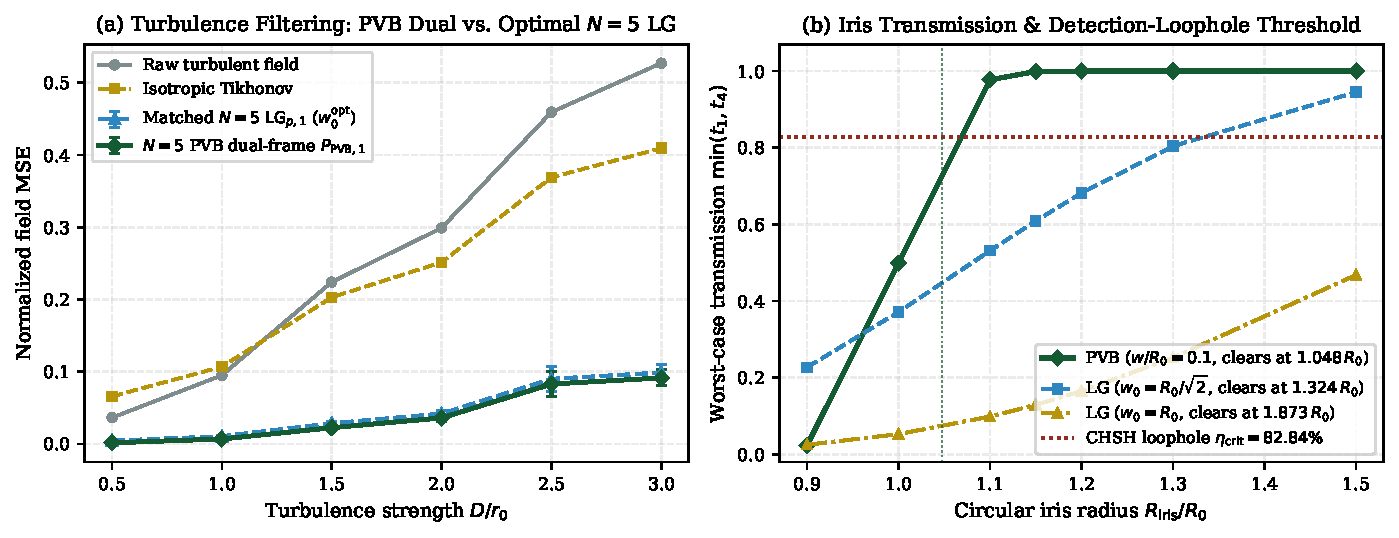
\includegraphics[width=\linewidth]{figures/fig1_p2_feasibility.pdf}
\caption{Key V15 Paper~2 feasibility proofs. (a)~Kolmogorov turbulence field MSE across $D/r_0 \in [0.5,3.0]$ showing the $N=5$ PVB dual-frame projector outperforming not only isotropic Tikhonov filtering but also an optimally waist-tuned matched-dimension $N=5$ $\mathrm{LG}_{p,1}$ radial projector. (b)~Worst-case single-photon iris transmission $\min(t_1,t_4)$ vs.\ $R_{\mathrm{iris}}/R_0$, showing PVB clearing the $82.84\%$ CHSH detection-loophole threshold at $1.048\,R_0$ while even $l=4$-matched LG requires $1.324\,R_0$.}
\label{fig:p2_feas}
\end{figure}

\paragraph*{Physical Discovery from the Parabolic GRIN RCF Solver.}
Solving the exact Sturm--Liouville problem for the parabolic GRIN profile $n_{\mathrm{GRIN}}^2(r) = n_{\mathrm{clad}}^2 + (n_{\mathrm{core}}^2 - n_{\mathrm{clad}}^2)\max(0, 1 - [(r-r_{\mathrm{mid}})/a_{\mathrm{ring}}]^2)$ reveals that $l = 0\text{--}6$ are strictly guided ($n_{\mathrm{eff}}(6) = 1.44760 > n_{\mathrm{clad}} = 1.444$) whereas $l = 7, 8$ drop below cladding cutoff ($1.44295, 1.43777$) because the parabolic profile carries lower integrated core index-volume than a step-index ring of equal width. This explains from first principles why Villalba \emph{et al.}~\cite{Villalba2023} operated precisely over $l = 1\text{--}6$ in their GRIN RCF, while confirming $+6.97\,\mathrm{dB}$ PVB coupling gain at $l=4$ (within $0.14\,\mathrm{dB}$ of the experimental $+6.83\,\mathrm{dB}$).

\section{Verified Target Journal Formats and Sequential Release Plan}
\label{sec:p2_formats}

Table~\ref{tab:p2_journals} summarizes the verified zero-APC target journals and official 2026 LaTeX templates for V15 Paper~2. Crucially, **Paper~2 must be submitted only after Paper~1 receives its arXiv identifier**, replacing the temporary preprint citation \texttt{AyalaV15Paper1}~\cite{AyalaV15Paper1} with Paper~1's live arXiv ID.

\begin{table}[t]
\centering
\caption{Verified 2026 LaTeX formats, costs, and peer-review models for V15 Paper~2 (standalone classical \& quantum photonics).}
\label{tab:p2_journals}
\scriptsize
\renewcommand{\arraystretch}{1.15}
\begin{tabularx}{\linewidth}{@{}l>{\raggedright\arraybackslash}p{3.1cm}>{\raggedright\arraybackslash}p{2.4cm}>{\raggedright\arraybackslash}p{2.4cm}>{\raggedright\arraybackslash}X@{}}
\toprule
\textbf{Journal (Publisher)} & \textbf{Official 2026 LaTeX Class} & \textbf{Mandatory Fee} & \textbf{Peer Review} & \textbf{Strategic Fit for Paper~2} \\
\midrule
\rowcolor{greenbg}
\textbf{\emph{Journal of Optics}} (IOP) & \texttt{iopjournal.cls} (\texttt{[anonymous]} option) & \textbf{\$0} (hybrid subscription) & \textbf{Double-anonymous} & \textbf{Top Choice (\#1):} Native home for combined classical + quantum structured-light applications (\texttt{Ferreira2026}, \texttt{Reddy2016}); removes solo-author affiliation bias. \\
\rowcolor{greenbg}
\textbf{\emph{JOSA B}} (Optica) & \texttt{optica-article.cls} (\texttt{\textbackslash journal\{opticajournal\}}) & \textbf{\$0 up to 10 pp} (\$300/pp $>10\,$pp) & Single-anonymous & \textbf{Strong Choice (\#2):} Currently $\sim 8$--$9$ pp (comfortably $\le 10\,$pp \$0 threshold); ideal if emphasizing Protocols~3--4 (quantum tomography \& CHSH). \\
\textbf{\emph{Optics Communications}} (Elsevier) & \texttt{elsarticle.cls} & \textbf{\$0} (hybrid subscription) & Single-anonymous & Reliable zero-APC structured-light backup (\texttt{Gori1987} Bessel--Gauss classic). \\
\bottomrule
\end{tabularx}
\end{table}

\section{Pre-Drafting Checklist and Approval Gate}
\label{sec:p2_gate}

All prerequisites for V15 Paper~2 are complete for your review: (i)~17 downloaded open-access arXiv PDFs and 37-entry clean \texttt{references\_v15\_paper2.bib}; (ii)~this Feasibility Analysis documenting all four referee-proofing upgrades; and (iii)~the complete pen-and-paper manual (\texttt{V15\_Paper2\_Step\_by\_Step\_Derivations.pdf}) verified by \texttt{verify\_paper2\_v15.py}. Upon your approval of both Feasibility Analyses and both Step-by-Step Derivation manuals (and confirmation of target formats: e.g., \emph{JOSA A} or \emph{J.\ Phys.\ A} for Paper~1, and \emph{Journal of Optics} or \emph{JOSA B} for Paper~2), we will proceed to draft V15 Paper~1 and V15 Paper~2 in their official publisher templates.

\bibliographystyle{unsrtnat}
\setlength{\bibsep}{1.8pt}
{\footnotesize
\bibliography{../References/references_v15_paper2}
}

\end{document}
